%!TEX root = ../Thesis.tex
\chapter{Genetic markers of hub connectivity in the human brain}
\label{ch:Chapter5}
\fancyhead[R]{\textit{Chapter.} \textit{\thechapter: }\textit{Genetic markers of hub connectivity in the human brain}}

\textbf{Aurina Arnatkevi\u{c}i\={u}t\.{e}},
Stuart Oldham,
Ben D. Fulcher,
Mark Bellgrove,
Alex Fornito.
Genetic markers of hub connectivity in the human brain. \textit{This manuscript is currently in preparation}.\\

\section*{Preamble}
The ultimate goal of this thesis is to investigate genetic markers of hub connectivity across different scales. Building on the previous work in the mesoscale \citep{Fulcher2016} and microscale [\citep{Arnatkeviciute2018}, presented in Chapter 2] connectomes, we next aimed to comprehensively examine the genetic markers of hub connectivity in the human brain through combining diffusion weighted imaging, genotyping, and AHBA gene expression data. In this chapter we investigated edge-wise, connectome-wide heritability, the effects of structural DNA variation through the polygenic scores, and the transcriptional signature of hub regions. We show that connectivity between hubs is the most highly heritable, is related to polygenic liability for mental illness, and high IQ. We also show that hubs in the human brain have elevated transcriptional coupling that is predominantly driven by metabolism-related genes, mirroring previous findings in mouse \citep{Fulcher2016} and human \citep{Vertes2016b}. Together, this work establishes a link between molecular function and large-scale connectome organization and demonstrate that the genetic influences on brain network organisation converge on hubs.\\
Supplementary materials for this chapter are in Appendix \ref{appendixC}.

\newpage

\section*{Abstract}
Nervous systems characteristically possess a relatively small number of highly connected regions, called network hubs, that are also highly interconnected with each other, forming a so-called `rich club’. Rich club organization plays an important role in supporting integrated brain function and is highly conserved, having been identified in diverse species with varying biological complexity. Such conservation points to a potential role of genes in shaping hub connectivity. Here, we comprehensively investigate genetic markers of hub connectivity in the human brain, as measured using diffusion MRI, by characterising its heritability, polygenic basis, and transcriptional signature. Using connectome-wide heritability analysis of 117 MZ and 60 DZ twin pairs, we demonstrate that the integrity of connections between hubs are under the strongest genetic control compared to hub--non-hub and non-hub--non-hub connections. At the level of structural DNA variation, we demonstrate that higher polygenic liability for psychiatric disorders is associated with reduced structural integrity of hub--hub connections, whereas higher polygenic scores for IQ are related to increased hub connection strength. Using gene expression data from the Allen Human Brain Atlas (AHBA), we show that hub regions display  tightly coupled transcriptional profiles, and that this effect is driven most strongly by genes regulating energy metabolism, mirroring results in the mesoscale mouse connectome \citep{Fulcher2016}. Together, these findings suggest that connections between hubs are under strong genetic influence with genetic variants driving this effect implicated in risk for mental illness and inter-individual differences in intelligence. Moreover, we show that hub regions are characterised by a distinct and highly conserved transcriptional signature defined by elevated coupling of metabolic gene expression.

\section{Introduction}

Nervous systems are complex, intricately connected networks that show non-trivial organisation over multiple spatial and temporal scales. The underlying wiring principles that lead to this complex organization however are still not well understood. The most general and longest-standing principles were first proposed by Santiago Ram\'{o}n y Cajal over a hundred years ago, who stated that neurons and their processes are configured to conserve time, space, and material \citep{RamonyCajal1995}. Conservation of space and material refers to a minimization of cellular and physical resources (e.g., dense cell packing, minimal axonal length) whereas conservation of time refers to the establishment of efficient networks that enable rapid communication between neural elements.

Since Cajal's initial proposal, most research has focused on the conservation of space and material. This work has shown that the minimization of network cost, often measured in terms of axonal wiring volume, can explain many features of neuronal organisation \citep{Cherniak1994,Chklovskii2002,Klyachko2003,Rivera-Alba2011,Wen2005}, ranging from the geometry of neuronal arbors \citep{Cherniak1999} to the placement of cortical areas \citep{Cherniak2004}. However, if the connection costs were strictly minimised, nervous systems would resemble a lattice, forming only short-range connections. But this is not the case, instead, brain networks possess more long-range connections than would be expected under a pure cost-minimisation model \citep{Bassett2006,Bullmore2012,Kaiser2006}. It is thought that these long-range connections act as shortcuts to facilitate communication between distant brain regions, thereby increasing topological integration within the network \citep{Bullmore2012,Buzsaki2004a,VandenHeuvel2012} and supporting adaptive, functional complexity \citep{Betzel2018}. These considerations suggest that nervous systems are configured to optimise a trade-off between the minimisation of wiring cost on one hand and the optimization of communication efficiency, integration and functional complexity on the other \citep{Bullmore2012}. This trade-off is consistent with Cajal's conservation laws, such that minimization of wiring costs minimises `material and space', whereas minimization of communication delays conserves `time'.

A key factor in how nervous systems negotiate the trade-off between conservation of material and time depends on precisely where the long-range connections of the system are formed. Numerous studies of connectomes, acquired in diverse species and measured at different resolution scales, have shown that these long-range connections are preferentially located between highly connected network elements called hubs \citep{Harriger2012,Towlson2013,VandenHeuvel2011,VandenHeuvel2013b}. Indeed, brain hubs are more strongly interconnected with each other than expected by chance, forming a so-called rich club, and the connections between hubs account for a disproportionate fraction of neuronal wiring costs \citep{Arnatkeviciute2018,Fulcher2016,Harriger2012,Towlson2013,VandenHeuvel2011}. Connections between hubs also mediate a large fraction of signal traffic in the brain \citep{Misic2016,VandenHeuvel2011}, indicating that the brain rich club represents a costly yet critical communication backbone for integrated  functioning \citep{Gratton2012,Markov2013a,VandenHeuvel2018,VandenHeuvel2013a}. Rich club organisation has been identified in the microscale neuronal connectome of the \textit{C.elegans} \citep{Towlson2013}, the mesoscale connectomes of the mouse \citep{Fulcher2016}, rat \citep{Liang2017}, cat \citep{DeReus2013b}, and macaque \citep{Harriger2012}, and the human connectome as measured at the macroscale with diffusion MRI \citep{VandenHeuvel2011}. This strong conservation of the rich club organisation across species suggests that genes may play a central role in shaping hub connectivity.

Several methods are now available to understand how genes shape brain connectivity \citep{Lein2017,Luo2018}. In humans, the three most commonly employed involve: i) quantitative modelling of heritability using twin pairs  \citep{Jansen2015}; ii) testing for correlations between phenotypic and allelic variation of the genome using either candidate gene, genome-wide, or polygenic associations \citep{Thompson2013}; and iii) testing for associations between network properties and anatomical variations in gene expression using publicly available expression atlases \citep{Fornito2019}.

Each of these genetic approaches is complementary. Heritability analyses rely on the inherent genetic differences between monozygotic (MZ) and dizygotic (DZ) twin pairs. Assuming that MZ twins share a 100\% of their genes whereas DZ twins, on average, share 50\% of their genes, it is possible to use structural equation models to determine the proportion of trait variance that is attributable to genetic factors. Several twin studies have investigated the heritability of various connectivity related phenotypes \citep{Bohlken2014,Colclough2017,Fu2015,Shen2014,Sudre2017}, but none have investigated hub connectivity directly. One early small sample size study found that cost-efficient properties of functional connectivity in human brain networks were strongly heritable, particularly in areas of association cortex, which are known to be brain network hubs \citep{Fornito2011}.

One limitation of the twin design is that it does not identify the specific genes or variants that mediate heritability. This limitation can be overcome by testing for associations between trait and allelic variation at multiple alleles scattered throughout the genome. Early candidate gene studies showed poor reproducibility \citep{Hutchison2004,Sullivan2007}, so more recently there has been a major investigation in genome-wide association studies (GWAS) which use very large samples to test for associations at millions of allelic markers throughout the genome \citep{Bush2012}. As an extension of this work, polygenic scores for GWA-investigated traits can be estimated, which aggregate an individual’s net genetic liability for a given phenotype \citep{Torkamani2018}. In the context of brain connectivity, a number of early candidate gene studies found relationships between selected genes and white matter microstructure \citep{Braskie2012,Chiang2011,Jahanshad2012b}, topological network properties \citep{Dennis2011}, and resting state functional connectivity \citep{Filippini2009,Trachtenberg2012,Westlye2011}. Variants related to structural connectivity \citep{Chiang2009,Jahanshad2012a,Jahanshad2013} and a broad set of imaging phenotypes \citep{Elliott2018} have been later identified through the data-driven GWAS. Building on the prior disorder-related GWAS, polygenic scores for a set of psychiatric disorders have been related to cortical gyrification \citep{Liu2016a}, functional connectivity \citep{Dezhina2018,Sadeh2018,Wang2017}, and longitudinal changes in white matter properties \citep{Alloza2018}. However, the functional effects of statistically-identified variants may be unclear such that these variants may not be causal, as GWAS can detect an association to a nearby tag variant that does not in itself exert a causal influence on the phenotype \citep{Wang2010}.

A third approach that more directly bridges the gap between gene function and phenotype relies on recently constructed brain-wide gene expression atlases \citep{Hawrylycz2012} [for a review see \citep{Keil2018}]. Gene expression provides a direct measure of the degree to which a gene has been transcribed in a given tissue and may thus be more proximally related to the functional effects of key genes than statistically-identified DNA variants. However, current human gene expression atlases are constructed from post-mortem data, meaning that we can only examine how anatomical variations in the expression patterns of a gene correlate with spatial variations in a given neural phenotype and cannot understand individual phenotypic variability in this context \citep{Fornito2019}. Moreover, gene expression, commonly quantified through messenger RNA (mRNA) abundance, provides only an indirect marker of the actual abundance of the protein in the cell [\citep{Futcher1999,Greenbaum2003,Gygi1999}, for other limitations of this approach see \citep{Fornito2019}]. Nonetheless, converging evidence from atlas-based studies suggest that brain network hubs carry a distinctive transcriptional signature \citep{Arnatkeviciute2018,Fulcher2016,Rubinov2015c,Vertes2016b}. An atlas-based analysis of the mouse connectome found that connected pairs of hubs show increased transcriptional coupling, defined as the similarity in the gene expression profiles between brain regions, relative to hub--non-hub and non-hub--non-hub connections, with the effect being primarily driven by genes regulating oxidative synthesis and metabolism of ATP \citep{Fulcher2016}. Notably, elevated transcriptional coupling of hubs was apparent despite hubs being separated by longer anatomical distances, on average, than other pairs of areas, which showed a strong tendency for reduced transcriptional coupling as a function of anatomical separation. Increased gene expression similarity between hubs has also been replicated in the microscale connectome of \textit{C.elegans} nervous system \citep{Arnatkeviciute2018}. Similarly, a separate study of functional hub connectivity in the human brain found that regions with long-range connections predominantly linking different modules tend to have higher expression of genes regulating oxidative metabolism and mitochondrial function \citep{Vertes2016b}. Spatial patterning of gene expression has also been associated with hubs in development \citep{Whitaker2016a} and disease \citep{Rittman2016}. Together, these findings suggest that hub regions across different species and scales exhibit transcriptional properties that are related to their high metabolic demands.

Here, we aim to comprehensively investigate genetic markers of hub connectivity by examining its heritability, polygenic influences and transcriptional correlates in the human connectome. We hypothesised that if hub connectivity and rich club organization is a highly conserved feature of brain organization, then connections between hubs should be strongly heritable. Moreover, if hub connectivity supports integrated function and is susceptible to disease \citep{Crossley2016a,Fornito2015}, then individuals with high polygenic scores for mental illness should show weaker hub connectivity, whereas individuals with high polygenic scores for IQ should show stronger hub connectivity. Finally, given prior findings in the mouse \citep{Fulcher2016} and worm \citep{Arnatkeviciute2018}, we predicted that connected pairs of hubs should show elevated transcriptional coupling compared to other areas, and that this effect will be driven by genes regulating metabolism-related processes.

\section{Materials and methods}

To comprehensively investigate genetic influences on hub connectivity we combined three different data modalities: structural brain connectivity derived from the DWI, brain-wide gene expression from the AHBA, and polygenic scores for IQ and several psychiatric disorders. These multimodal data allowed us to assess the relationship between brain connectivity and genetics in different ways: quantitatively, through the edge-wise, connectome-wide heritability analysis; at the level of gene expression; at the level of structural DNA variation through polygenic score (PGS) analysis; and through the analysis of the correlated gene expression (CGE) patterns (Figure \ref{fig:Ch5Fig1}).

\begin{figure}[h!]
\begin{center}
\includegraphics[width=1\textwidth]{Chapter5/Ch5Fig1.pdf}% This is a *.eps file
\end{center}
\caption{\textbf{Schematic: investigating the genetic markers of hub connectivity.}
A) A schematic representation of the connectome illustrating different connection types in the brain: rich – connections between two hubs; feeder – connections between a hub and a non-hub; peripheral – connections between two non-hubs. 
B) heritability analysis using structural equation modelling is applied to every connection within the brain (ACTE model illustrated). Mean heritability estimates are then compared across rich, feeder, and peripheral connections; 
C) connection weights for each link across subjects are correlated with polygenic scores for a range of psychiatric disorders and for IQ. The average correlation value across link types is then compared between link types. Rich links are expected to show a stronger negative relationship for disorders and a stronger positive relationship for IQ compared to other links within the brain. Sample data are shown for visualisation purposes. D) gene expression data from the AHBA shown as a region $\times$ gene matrix. Region-specific vectors of expression values across all genes are then correlated between all pairs of regions, yielding a measure of transcriptional coupling, or correlated gene expression (CGE). Average CGE values are then compared across rich, feeder, and peripheral links.}
\label{fig:Ch5Fig1}
\end{figure}

\subsection*{Diffusion weighted imaging}
\label{sec:DWI}

The DWI data used to define the structural connectivity network were obtained from two separate sources: the Human Connectome Project [HCP, \citep{VanEssen2013}] and a study conducted at Monash University (Monash Cohort). We used the minimally processed DWI and structural data from the HCP for 972 participants ($age_\mathrm{mean} = 28.7 \pm 3.7$, 522 females), including a cohort of related individuals –-- MZ and DZ twin pairs together with their non-twin siblings (more details presented in the \nameref{sec:Heritability} section). HCP data were acquired on a customized Siemens 3T ``Connectome Skyra'' scanner at Washington University in St Louis, Missouri, USA using a multi‐shell protocol for the DWI: 1.25 mm$^{3}$ isotropic voxels, repetition time (TR) = 5520 ms, echo time (TE) = 89.5 ms,  field-of-view (FOV) of 210 $\times$ 180 mm, 270 directions with b = 1000, 2000, 3000 s/mm$^{2}$ (90 per b value), and 18 b = 0 volumes. Structural T1-weighted data were collected using 0.7 mm$^{3}$ isotropic voxels, TR = 2400 ms, TE = 2.14 ms, FOV of 224 $\times$ 224 mm. The full details can be found elsewhere \citep{Glasser2013}.

The Monash Cohort comprised 414 participants with MRI data obtained on a Siemens Skyra 3T scanner at Monash Biomedical Imaging in Clayton, Victoria, Australia using the following DWI parameters: 2.5 mm$^{3}$ voxel size, TR = 5520 ms, TE = 89.5 ms, FOV of 210 $\times$ 180 mm, 60 directions with b = 3000 s/mm$^{2}$, and seven b = 0 volumes. T1-weighted structural scans were acquired using: 1 mm$^{3}$ isotropic voxels, TR = 2400 ms, TE = 2.14 ms, FOV of 224 $\times$ 224 mm. Data for 82 subjects were excluded due to low connectome density (n = 11, connectome density more than 3 standard deviations lower than the mean) or no genotype data (n = 71), resulting in a sample of 332 participants ($age_\mathrm{mean} = 23.7 \pm 5.5$, 189 females).

Pre-processing for T1-weighted structural images in the Monash Cohort consisted of visual screening for gross artefacts followed by the reconstruction of grey/white matter interface and the pial surface using FreeSurfer v5.3.0 software. Surface reconstructions for each subject were visually inspected, performing manual corrections as needed to achieve a more accurate surface representation. Network nodes for each individual in both datasets were defined using a recently-developed, data-driven group average parcellation of the cortex into 360 regions (180 per hemisphere) \citep{Glasser2016}. To ensure that our results were not driven by the use of this parcellation, we also replicated our findings using a random cortical parcellation consisting of 500 approximately equally sized regions (250 per hemisphere) that was generated by randomly subdividing anatomical Desikan-Killiany parcellation \citep{Desikan2006}. The advantage of this parcellation is that it minimizes differences in size between regions, which can bias results.

Subsequent processing of the DWI data for both datasets was performed using the MRtrix3 \citep{Tournier2012} and FMRIB Software Library \citep{Jenkinson2012}. Tractography was conducted in each participant's T1 space using second order integration over fibre orientation distributions (iFOD2), a probabilistic algorithm that improves the quality of tract reconstruction in both highly curved and crossing-fiber regions \citep{Tournier2010}. To further improve the biological accuracy of the structural networks we also applied Anatomically Constrained Tractography (ACT), which delineates the brain into different tissue types (cortical grey matter, subcortical grey matter, white matter, cerebrospinal fluid) and uses that information to ensure that streamlines are beginning, traversing, and terminating in anatomically plausible locations \citep{Smith2012}. A total of 10 million streamlines were generated on a probabilistic basis using a dynamic seeding approach that evaluates the relative difference between the estimated fibre density and current streamline reconstruction, and preferentially samples from areas of insufficient density \citep{Smith2015a}.

The resulting tractogram was then combined with the cortical parcellation for each subject to produce a network map of white matter connectivity. Streamline termination points were assigned to the closest region within a 5 mm radius. Connection weights were quantified using streamline count (number of streamlines connecting two regions, SC), as well as the mean fractional anisotropy (FA) of voxels traversed by streamlines connecting two regions. Streamline count provides a measure of relative connection strength derived from the tractography algorithm, whereas FA acts as a marker of the white matter microstructure along the tract; both measures are subject to certain caveats \citep{Jones2013}.
Connectomes derived from probabilistic tractography algorithms are often thresholded due to the high probability of false-positive connections \citep{Sarwar2019,Sotiropoulos2017}. Commonly used methods involve a range of options including weight-based, consistency-based and density-based thresholding approaches \citep{Betzel2018,Roberts2016a}: weight-based thresholding eliminates connections below a particular threshold; consistency-based thresholding retains connections present in a set proportion of subjects; and density-based thresholding retains connections based on a particular property (weight, consistency, or other) to achieve a desired connectome density. No consensus has been reached regarding the most appropriate thresholding method. In our analysis, we combined consistency-based and density-based approaches, selecting edges that are commonly reconstructed across subjects and then deriving a group-representative connectome at a specified density. This resulted in a single group-average connectome for the HCP and Monash datasets. Specifically, we: i) selected edges that are present in at least $30\%$ of subjects; and ii) retained the strongest edges (based on the streamline count) to achieve the desired connectome density. Since the desired connection density is arbitrary, we examined our results across a range of densities to evaluate the sensitivity of our findings. For the 360 region parcellation, we considered $15\%$, $20\%$, $25\%$ densities. Given the higher number of possible connections using a higher resolution parcellation of 500 regions, we evaluated slightly lower densities: $10\%$, $15\%$, and $20\%$.

The group-representative connectome derived from the HCP dataset was then used as a binary mask for selecting edges for the heritability and gene expression analyses, while the group-representative connectome derived from the Monash dataset was used for selecting edges for the polygenic score (PGS) correlation analyses. We chose to define connections for the gene expression analysis based on the HCP connectomes due to the higher sample size and superior data quality. In both heritability and PGS analyses, we quantified connection weights using FA and SC. We focus on results for the former and present results for the latter in Appendix \ref{app:AppendixCh5_2}. To enable a more direct comparison to the previous analyses of gene expression in mouse \citep{Fulcher2016} and \textit{C.elegans} \citep{Arnatkeviciute2018}, our gene expression analysis in human was performed using binary connectivity matrices where connections with non-zero weights in a group-representative matrix are labelled as present. 


\subsection{Network analysis}
In this section we outline the network analysis methods that were used to characterize structural brain connectivity.

\paragraph*{Degree and strength.}

The connectivity of each region (node) in a network can be quantified by counting the number of connections that a node has, known as degree, \textit{k}. At a particular degree threshold, \textit{k}, nodes can be labelled as hubs (degree $> k$) or non-hubs (degree $\leq k$). Subsequently, all connections within the network can be classified as `rich' (between two hubs), `feeder' (between a hub and a non-hub), and `peripheral' (between two non-hubs). In a weighted network, a node can be also characterised by summing the total weight of its connections, known as node strength.

\paragraph*{Rich club organisation.}

To quantify the interconnectivity between hub regions within a binary brain connectivity network, we used the topological rich club coefficient $\phi(k)$:

\begin{equation}
    \label{eqn:Ch5Eq1}
    \phi(k) = \frac{2E_{>k}}{N_{>k}(N_{>k}-1)},
\end{equation}

where $N_{>k}$ is the number of nodes with degree $>k$, and $E_{>k}$ is the number of edges between them \citep{Colizza2006}. Therefore, the rich club coefficient quantifies the density of the subgraph consisting of nodes with degree higher than a selected threshold \textit{k}. Nodes with higher degree make more connections, resulting in a higher expected connection density between them. To quantify levels of connectivity in excess of this, we compared the $\phi(k)$ in the empirical network to the mean value across a 1000 randomized null networks, $\phi_\mathrm{rand}(k)$, that were generated by rewiring the edges in the empirical network while retaining the same degree sequence, using the \texttt{randmio\_und} function from the Brain Connectivity Toolbox \citep{Rubinov2010}. Each edge was rewired on average of 50 times per null network.

To assess whether the connections between high-degree nodes in a weighted network were more likely to have stronger weights than expected by chance, we also evaluated the weighted rich club coefficient \citep{Opsahl2008}:

\begin{equation}
    \label{eqn:Ch5Eq2}
    \phi^{w}(k) = \frac{W_{>k}}{\sum_{l=1}^{E_{>k}}w^\mathrm{rank}_{l}},
\end{equation}

where $W_{>k}$ is the sum of weights in the sub-graph with degree higher than \textit{k}, and the denominator is the total sum of \textit{l} strongest weights in the network. Separating the definitions of weighted and topological rich club coefficients, instead of rewiring the links, here we randomly reassigned weights within the network while preserving the binary topology of the network  \citep{Alstott2014}. In both cases, we computed the normalised rich club coefficient $\phi_\mathrm{norm}(k)$ as the ratio between the rich club coefficient in the empirical network and the mean rich club coefficient in the set of the corresponding randomised networks:
\begin{equation}
    \label{eqn:Ch5Eq3}
    \Phi_\mathrm{norm}(k) = \frac{\phi(k)}{\langle \phi_\mathrm{rand}(k) \rangle}.
\end{equation}
Values of $\Phi_\mathrm{norm}$ exceeding 1 indicate rich club organisation, where high degree nodes are more densely interconnected (in a case of the topological rich club) or have higher weights (in a case of the weighted rich club) than be expected by chance. The statistical significance of the result is assessed by computing a $p$-value directly from the empirical null distribution of the 1000 randomised networks, $\phi_\mathrm{rand}(k)$, as a permutation test \citep{VandenHeuvel2011}.

\paragraph*{Communicability.}

Connections that mediate a high proportion of traffic within the brain are critical for information transfer. To confirm that this was the case in our data, and considering that neuronal signals within brain networks may not necessarily propagate along shortest topological paths, we investigated the topological centrality of rich links using a measure called communicability \citep{Estrada2008} across a range of degree thresholds. The communicability $C_{ij}$ between a pair of nodes \textit{i} and \textit{j}, is calculated accounting for all possible paths of length \textit{l} between the nodes, weighted as $1/l!$, so that shorter paths are assigned higher weights and consequently have a higher contribution to the overall score. The communicability, $C_{ij}$, for a binary matrix A is formally defined as:
\begin{equation}
    \label{eqn:Ch5Eq4}
    C_{ij}= \sum_{l=0}^{\infty}\frac{(A^{l})_{ij}}{l!} = (e^{A})_{ij}.
\end{equation}

\subsection{Heritability analysis}
\label{sec:Heritability}

The HCP dataset includes 117 pairs of genetically confirmed monozygotic (MZ) twin pairs together with 82 of their non-twin siblings, as well as 60 dizygotic (DZ) same-sex twin pairs and 58 of their non-twin siblings. For each twin pair with more than one non-twin sibling, one sibling was selected at random (demographic details summarized in the Table \ref{Ch5Table1}). Only twin pairs where both twins had genotyping-verified zygosity were included in the heritability analysis.

\begin{table}[h!]
\centering
\caption{Demographic data for twin groups and their non-twin siblings. MZ -- monozygotic twins, DZ -- dizygotic twins. Age is displayed in years: mean $\pm$ SD.}
\label{Ch5Table1}
\begin{tabular}{@{}llll@{}}
\toprule
\textbf{Zygosity} & \textbf{Number of subjects} & \textbf{Sex (F/M)} & \textbf{Age} \\ \midrule
MZ twins & 117 pairs & 69/48 & $29.3 \pm 3.3$ \\
MZ non-twin siblings & 69 & 34/35 & $29.1 \pm 4.2$ \\
DZ twins & 60 pairs & 33/27 & $28.8 \pm 3.5$ \\
DZ non-twin siblings & 48 & 24/24 & $29.1 \pm 4.0$ \\ \bottomrule
\end{tabular}
\end{table}

Heritability analysis relies on the assumption that the similarity in a particular trait between twins is due to the additive effects of shared genes or shared environmental factors. While MZ twins share all their genes and therefore are genetically identical, DZ twins on average share half of their genes resulting in 50\% genetic similarity (similar to non-twin siblings). Whereas shared genetic factors as well as common environment contribute to the similarity between twins in a pair, unique environmental factors contribute to the differences observed between them. Therefore, it is possible to decompose the phenotypic variance and covariance in any particular trait into several factors such as additive genetic (A), common environmental (C) and unique environmental (E) influences. Considering that twins raised together might have experienced a more similar environment compared to their non-twin siblings, including a set of non-twin siblings into the analysis allows us to separate the common environmental contributions into twin-specific (T) and twin non-specific (C) common environment.

Structural equation modelling (SEM) was implemented for every connection in the group-averaged cortical connectome using OpenMx software \citep{Boker2011,Neale2016} in $R$. The main analysis was performed on the 360 region \citep{Glasser2016} cortical connectome (further referred as f360 parcellation) at $20\%$ density using fractional anisotropy as a connection weight. The analyses were subsequently reproduced with varying connectome densities ($15\%$ and $25\%$) and using a higher resolution random cortical parcellation [500 regions (further referred as r500 parcellation): $10\%$, $15\%$ and $20\%$ densities]. A range of biometric models -- ACTE, ACE, AE, CE, E -- were implemented in order to find maximum likelihood estimates of additive genetic (A), twin-specific common environmental (T), twin non-specific common environmental (C) and unique environment (E) factors using age and sex as covariates. Outlying connection weight values for each analysis were removed using the boxplot function in $R$ by keeping data points ($w$) in a range $Q1-1.5 \times IQR< w <Q3+1.5 \times IQR$ where $Q1$ and $Q3$ are the first and third quantiles respectively and $IQR$ is the interquartile range. The Akaike information criterion (AIC) \citep{Akaike1998} was used to compare the goodness of fit of all tested models in order to find the most parsimonious one. For each edge, the model with the lowest AIC was selected. Consequently, the narrow-sense heritability [the proportion of variance attributable to additive genetic factors (referred as heritability through this work)] was estimated for each connection using the best-fitting model.

\subsection{Genotype data}

DNA samples for 715 individuals of European descent from the Monash Cohort were genotyped using the Illumina Infinium PsychArray-24v1.2 BeadChip at Path West’s Diagnostic Genomics Laboratory in Western Australia. The Illumina Psych-Chip comprising of \num{510000} markers: \num{265000} tagging SNPs from the Infinium Core-24 BeadChip and \num{245000} markers from the Infinium Exome-24 BeadChip. Illumina Psych-Chip was developed in collaboration with the Psychiatric Genomics Consortium (PGC) and supplemented with an additional \num{50000} SNPs implicated in psychiatric and neurodevelopmental disorders.

We performed quality control (QC) using PLINK 1.9 software at both the individual subject and SNP level. Initially, we removed subjects with very low-genotyping score ($\geq 0.10$ of missing data) and excluded SNPs with genotyping call rate $<90\%$ and with a minor allele frequency (MAF) $< 0.01$. Further, several subject-level QC steps were performed by removing individuals: i) with disparities between the recorded and observed sex status as determined through X-chromosome homozygosity; ii) with low genotyping score ($\geq 0.05$ of missing data); iii) with cryptic relatedness higher than 0.25; iv) displaying outlying mean heterozygosity (greater than $\pm3$ SDs from the sample mean). In order to identify any potential sources of population stratification in the sample we performed multidimensional scaling (MDS) using HapMap3 dataset \citep{Consortium2010} and excluded subjects exceeding $\pm±2$SD on the $1st$ or $2nd$ principal components, leaving a total of 666 subjects for the imputation. SNPs with low genotyping call rate $<95\%$, MAF$<0.01$ and significantly departing from Hardy– Weinberg (H–W) equilibrium ($p<10^{7}$) were excluded leaving \num{283 616} variants in the final set taken forward to imputation. We used MaCH and Minimac2 for phasing and genotype imputation respectively employing the 1000 Genomes (phase one release three) reference panel. After imputation, SNPs with MAF$<0.01$ and MAF$>0.98$ were removed. To eliminate poorly imputed variants, SNPs with imputation quality $r^{2} < 0.8$ were excluded, resulting in a total of \num{5723894} variants used for computing the polygenic scores.

\subsection{Polygenic score calculation}

Polygenic scores (PGS) for five major psychiatric disorders: schizophrenia, major depressive disorder, ADHD, bipolar disorder, and autism spectrum disorder (ASD) as well as IQ were calculated using the PRSice software package \citep{Euesden2015}. The PGS for each subject were estimated as a sum of risk alleles, weighted by their effect size as defined in the latest publicly available GWA study for each trait \citep{Neale2010,Ripke2014a,Ruderfer2018,Savage2018,AutismConsortium2017,Wray2018} while controlling for sex, age, age$^{2}$, age $\times$ sex interaction, and the  first four principal components extracted from the MDS analysis (to adjust for population stratification) as covariates. PGS are calculated by selecting SNPs based on their association with a trait in the base GWAS. Selecting an appropriate SNP significance threshold for PGS calculations poses an issue of balancing statistical power and the strength of the association with a trait. More stringent thresholds generate a smaller set of SNPs that are more likely to be truly associated with the trait of interest whereas more liberal thresholds might help to increase the statistical power while possessing a risk of selecting SNPs that have weak associations. Considering that we did not have reliable measures of disorder-specific traits in our sample and therefore could not select the most predictive threshold ($p_{T}$) for each disorder, we chose a $p_{T}<0.05$ to balance the statistical power of the estimated PGR and the number of SNPs included in the analyses \citep{Ripke2014a}. The number of selected SNPs varied in the range \num{15 000}--\num{40 000} SNPs, depending on the trait of interest.

\subsection{PGS correlation}

After selecting subjects that had both DWI and PGS data available ($n= 332$, $age_\mathrm{mean} = 23.7 \pm 5.5$, 189 females) we used a partial (Spearman) rank correlation to evaluate the relationship between connection weight and the PGS for ASD, ADHD, major depression, bipolar disorder, schizophrenia and IQ, while controlling for participant age and sex. For each connection in the representative group connectome defined using the Monash Cohort data, we extracted FA-based connection weight values across subjects (SC-based results are presented in the Appendix \ref{app:AppendixCh5_2}). In each correlation, subjects with connections with outlying values were filtered in a two-step procedure: i) only the subjects with an existing connection were retained; ii) among the existing connections, only links with weight ($w$) within the range of $Q1-1.5 \times IQR< w <Q3+1.5 \times IQR$ were selected. This resulted in the exclusion of a median of 15 subjects ($IQR = 28$) at each edge. In the case of SC-based connection weights, a median of 36 subjects ($IQR=39$) were excluded for any individual edge. As a result, partial rank correlation coefficients were estimated for every connection in the representative group connectome.

\subsection{Gene expression}
\label{secGeneExpression}

We used brain-wide gene expression data from the Allen Human Brain Atlas (AHBA), which consists of microarray expression measures in 3702 spatially distinct tissue samples taken from six neurotypical postmortem adult brains \citep{Hawrylycz2012}. Different brain regions were sampled across each of the six AHBA donors to maximize spatial coverage, resulting in approximately 400--500 tissue samples in each brain. The samples were distributed across cortical, subcortical, brainstem and cerebellar regions, and quantify the expression levels of over \num{20000} genes. Considering that only two out of six brains were sampled from both left and right hemispheres whereas the other four brains have samples collected only from the left hemisphere, we decided to focus our analyses on the left cortex only. For more details about the data see \citep{Hawrylycz2012}.

The processing of the gene expression data consisted of several steps, outlined in \citep{Arnatkeviciute2019}. Briefly, i) probe-to-gene annotations were updated using the Re-Annotator toolbox \citep{Arloth2015}; ii) intensity based filtering was applied in order to exclude probes that do not exceed background noise in more than 50\% of samples; iii) a representative probe for each gene was selected based on the highest correlation to RNA sequencing data in two of the six brains \citep{Miller2014a}; iv) gene expression samples were assigned to the regions-of-interest by generating donor-specific grey matter parcellations and assigning samples located within 2 mm of the parcellation voxels; v) gene expression measures within a given brain were normalised first by applying a scaled robust sigmoid normalisation [see \citet{Arnatkeviciute2019}] for every sample across genes and then for every gene across samples in order to evaluate the relative expression of each gene across regions, while controlling for donor-specific differences in gene expression [see \citet{Arnatkeviciute2019} for a validation]. Normalised expression measures in samples assigned to the same region were averaged within each donor brain and aggregated into a region by gene $\times$ matrix consisting of expression measures for \num{10027} genes over 180 (left hemisphere, HCP parcellation) and 250 regions (left hemisphere of the random parcellation) respectively. For more details, see the Appendix  \ref{app:AppendixCh5_1}.

\subsection{Transcriptional coupling}
\label{sec:CGE}

Using the brain-wide gene expression measures from the AHBA, we quantified transcriptional coupling between regions using a measure of correlated gene expression (CGE). We defined CGE as the Pearson correlation between the normalised expression measures of available genes after pre-processing ($n=\num{10027}$). As shown in Figure \ref{fig:Ch5Fig1} and described in \citep{Arnatkeviciute2019}, CGE exhibits a strong spatial autocorrelation that can be approximated as an exponential relationship with separation distance, where pairs of regions in close proximity to each other demonstrate much more similar expression patterns (higher CGE) compared to region pairs separated by longer distances. To investigate whether CGE differs between different topological classes of connections beyond any low-order spatial effect, we fit an exponential function with form $r(d)=Ae^{-d/n}+B$. The parameters $A = 0.64$, $B = -0.19$ and $n=90.4$ capture the trend well, allowing us to retain the residuals for further analysis (Figure \ref{fig:Ch5Fig2}), defined as $\widehat{CGE_{ij}}=CGE_{ij} - r(d_{ij})$. These distance-corrected residual CGE values were used in all CGE analyses.

\begin{figure}[h!]
\begin{center}
\includegraphics[width=1\textwidth]{Chapter5/Ch5Fig2.pdf}% This is a *.eps file
\end{center}
\caption{\textbf{Relationship between correlated gene expression (CGE) and regional separation distance (d).}
(A) Correlated gene expression as a function of the regional separation distance on the cortical surface. The red line represents an exponential fit, $r(d)=0.64e^{-d/90.4}-0.19$.
(B) CGE residuals after removing the exponential trend. CGE between pairs of regions are represented in grey dots and red dots represent the mean value in 25 equiprobable distance bins.}
\label{fig:Ch5Fig2}
\end{figure}

To evaluate transcriptional coupling for different connection types, for every edge within the connectivity matrix, we assigned a distance-corrected CGE measure. At each degree threshold, \textit{k}, for defining hubs (degree $>k$), we then computed an average CGE value for every link type (rich -- connection between two hubs, feeder -- connection between a hub and a non-hub, and peripheral -- connection between two non-hubs). Significant increases in the CGE for a given link type compared to the rest of the network were evaluated using a one-sided Welch's $t$-test ($P<0.05$).

To determine which functional gene groups contribute the most to any observed differences in CGE across different link types in the brain, we estimated the gene contribution scores (GCS) as previously shown in \citep{Fulcher2016} using the definition of the Pearson correlation coefficient:

\begin{equation}
    \label{eqn:Ch5Eq5}
    \widehat{CGE_{ij}} = CGE_{ij} - r(d_{ij}) = \frac{1}{N}\sum_{a=1}^{N}[\widetilde{g}_{i}^{a}\widetilde{g}_{j}^{a} - r(d_{ij})] = \frac{1}{N}\sum_{a=1}^{N}GCS_{ij}^{a},
\end{equation}
where N is the number of genes (N = \num{10 027}), $\widetilde{g}_{i}^{a} \widetilde{g}_{j}^{a}$ the product of the $z$-score normalised expression values for gene \textit{a} in regions \textit{i} and \textit{j}, and $r(d_{ij})$ is a previously defined spatial autocorrelation effect approximated as an exponential line (Figure \ref{fig:Ch5Fig2}). Therefore, the gene contribution score between a pair of regions \textit{i} and \textit{j} for a gene a was defined as $GCS_{ij}^{a}= \widetilde{g}_{i}^{a}\widetilde{g}_{j}^{a} - r(d_{ij})$.

We then assigned each gene a $t$-statistic quantifying the increase in GCS for rich compared to peripheral links, as these two groups constitute the most distinct link types: a high value indicates increased CGE in rich compared to peripheral links. These $t$-statistic measures were used in the enrichment analyses as gene scores for determining whether any functional gene groups were contributing towards the increase in CGE more than others.

\subsection{Enrichment analysis}
\label{sec:enrichment}
Gene enrichment analyses assess whether any functional gene groups are overrepresented in a set of genes. Every gene in our sample (n = \num{10027} genes) was assigned a $t$-statistic score quantifying its contribution towards the increase in GSC for rich links relative to peripheral. Using these scores, we aimed to determine which specific functional groups of genes contribute to the observed increase in correlated gene expression. Functional gene group analysis was performed using version 3.1.2 of ErmineJ software \citep{Gillis2010}. Gene ontology (GO) \citep{Ashburner2000} annotations were obtained from GEMMA \citep{Zoubarev2012} as \texttt{Generic\_human\_ncbiIds\_noParents.an.txt} on May 16, 2018. Gene Ontology terms and definitions were acquired from the \url{archive.geneontology.org/latest-termdb/go_daily-termdb.rdf-xml.gz} on May 16 2018. We performed gene score resampling (GSR) analysis on the $t$-statistic scores testing the biological process GO categories with 5 to 100 genes available using the mean $t$-statistic score across genes to summarise the GO category and applying full resampling with 106 iterations. Resulting $p$-values were corrected across \num{5987} GO categories using the false discovery rate (FDR) method of \citet{Benjamini1995}.

\section{Results}

We start by describing the general topological properties of the representative cortical group connectome derived from the HCP dataset (results for the Monash Cohort are presented in the \ref{app:AppendixCh5_3}) before progressing to analyses of (i) heritability; (ii) polygenic variation; and (iii) transcriptional coupling. The results presented in the main text are based on the structural connectivity data derived using a functionally-defined brain parcellation \citep{Glasser2016}. The main results are reproduced using a range of connectome densities and a high resolution 500-region random parcellation (see \ref{app:AppendixCh5_2}).

\subsection{Rich club organisation of the human brain}

We first describe the topological properties of the group-representative connectome comprising \num{12924} unique connections between 360 functionally defined regions \citep{Glasser2016}. The network was thresholded retaining the 20\% edges with the highest weights (see section \nameref{sec:DWI}). Subsequently, the mean FA values along each tract were used as connection weights serving as a marker for the white matter microstructure of that tract. For each region, we counted the number of connections attached to it, called node degree, \textit{k}. As shown in Figure \ref{fig:Ch5Fig3}, the degree distribution of the group-averaged connectome has a long-tail, consistent with the presence of a small number of highly connected regions. These nodes represent putative network hubs.

For each degree threshold (\textit{k}), we quantified the connectivity between regions with degree $> k$ to determine whether higher degree nodes tend to preferentially connect to each other, forming a rich club. Figure \ref{fig:Ch5Fig3}A demonstrates the variation of the normalised topological rich club coefficient $\Phi_{norm}$ across a range of degree thresholds, \textit{k}, at which hubs are defined (as regions with degree $> k$). Circles indicate a significant increase in link density among hubs in the empirical network relative to 1000 degree-preserving nulls (permutation test, $p < 0.05$). The topological rich club organisation ($\Phi_{norm} >1$) is evident between nodes in the tail of the degree distribution, particularly spanning $105< k <146$, that we call the topological rich club regime (note that estimates can be unstable in the extreme ends of the tail due to a limited number of samples). Through this work, we define hubs as regions with $k > 105$, corresponding to the degree threshold at which the normalised rich club coefficient shows a sharp and consistent increase at high \textit{k}.

\begin{figure}[h!]
\begin{center}
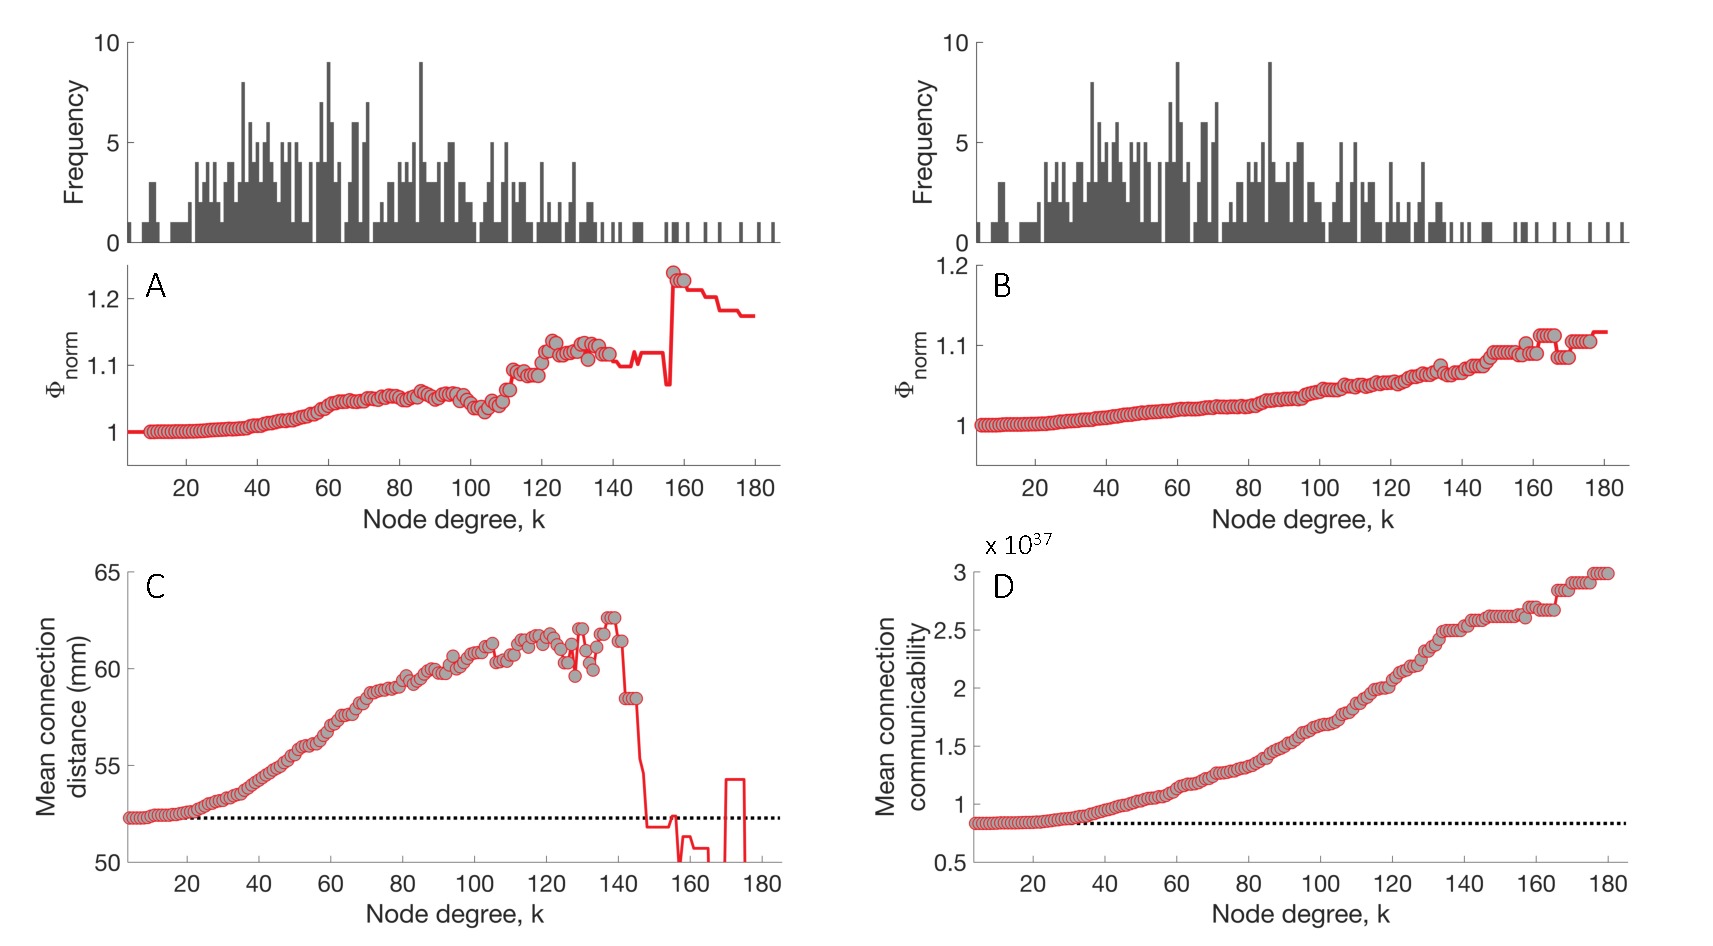
\includegraphics[width=1\textwidth]{Chapter5/Ch5Fig3.pdf}% This is a *.eps file
\end{center}
\caption{\textbf{Rich club organisation of the connectome.}
Top: the degree distribution of the connectome. Bottom:
(A) Normalized topological rich club coefficient $\Phi_{norm}$; $\Phi_{norm} >1$ indicates that hubs are more densely interconnected than expected by chance; circles indicate values that are significantly higher compared to an ensemble of 1000 degree-matched null networks ($p < 0.05$).
(B) Normalized weighted rich club coefficient ($\Phi_{norm}^{w}$); $\Phi_{norm}^{w}>1$ indicates that connections between hubs are stronger than expected by chance; circles indicate values that are significantly higher than an ensemble of 1000 topology-matched null networks ($p < 0.05$). Mean Euclidean separation distance between connected hub regions (C) and mean connection communicability (D) as a function of the degree, \textit{k}, at which hubs are defined (as regions with degree $> k$); The mean connection distance and communicability values across all network links shown as a dotted black line; circles indicate values significantly greater than across all other pairs of connected regions (right-tailed Welch’s $t$-test, $p < 0.05$).}
\label{fig:Ch5Fig3}
\end{figure}

Using the weighted rich club coefficient ($\Phi_{norm}^{w}$), we quantified whether connections between hubs tend to be stronger than expected by chance. In this analysis, the null networks were generated by randomising the connection weights while preserving the network topology. Such randomisations allow to assess the weighted rich club effect that is independent from the topological rich club \citep{Alstott2014}. The continuous increase in the weighted rich club coefficient across degree thresholds (Figure \ref{fig:Ch5Fig3}B) indicates that, in addition to being more densely interconnected as defined by the topological rich club, hub regions preferentially share stronger connections.

Compared to other connections within the network, connections between hubs display a higher mean connection length (Figure \ref{fig:Ch5Fig3}C). The high interconnectivity between hubs as well as their tendency to share stronger and longer distance connections indicate the high wiring-cost associated with establishing and maintaining hub connectivity. These properties counter the general trends across the brain observed in different species where connection probability \citep{Arnatkeviciute2018,Fornito2019,Fulcher2016} and weight \citep{Betzel2018} tend to decrease with distance.

The topological centrality of each edge serves as a proxy for its functional importance in network communication and can be quantified using a measure of communicability which accounts for the contribution of all possible paths between a pair of nodes [and is consistent with a diffusive model of signal propagation; see \citep{Avena-Koenigsberger2017}]. Here we show that the mean connection communicability increases as a function of degree (Figure \ref{fig:Ch5Fig3}D) suggesting that connections between hubs are likely to mediate a high proportion of signal traffic within the brain. Collectively, these results indicate that, rich links are particularly costly and functionally important elements of the connectome, as has previously been shown in human \citep{VandenHeuvel2011} and other species \citep{Arnatkeviciute2018,Fulcher2016,Towlson2013}. Having established the importance of hub connectivity we now turn to investigate the genetic correlates associated with hub connectivity.

\subsection{Heritability}

We start with quantifying the degree to which genes influence brain connectivity using a connectome-wide heritability analysis (see section \nameref{sec:Heritability}). Biometric models (ACTE, ACE, AE, CE, E) of individual variability in the connection strength were fitted to every edge to partition the phenotypic variability into several factors: additive genetic (A); common environmental (C); twin specific common environmental (T) and unique environmental (E). The best-fitting model for every edge was determined using the Akaike information criterion \citep{Akaike1998}. For the majority of connections, the selected model included the additive genetic component (AE $= 48\%$, ACTE $= 17\%$, ACE $<1\%$), while $34\%$ of connections did not display a significant genetic contribution (E $= 24\%$, CE $= 10\%$).

\begin{figure}[h!]
\begin{center}
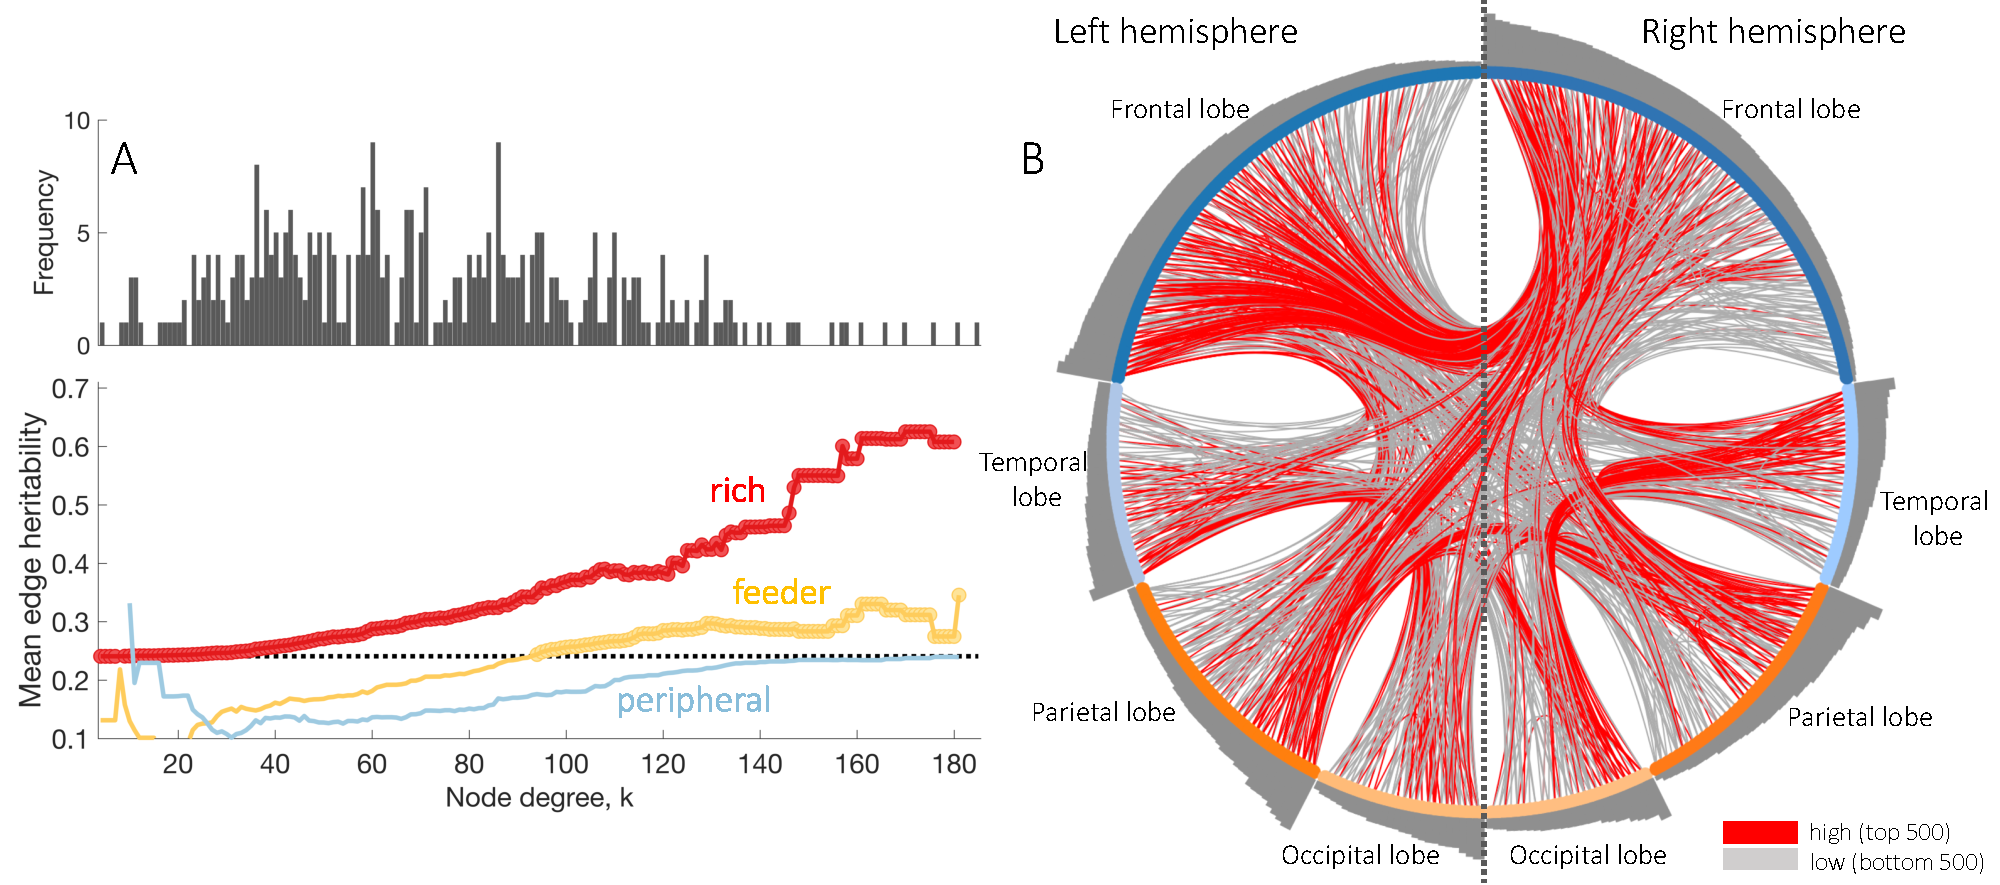
\includegraphics[width=1\textwidth]{Chapter5/Ch5Fig4.pdf}% This is a *.eps file
%https://immersive.erc.monash.edu/neuromarvl/?save=7ecb3a65-228e-4299-bcd4-2c65423741a8_130.194.90.94
\end{center}
\caption{\textbf{Rich links show an increased heritability.}
(A) Top: The degree distribution of the representative group-level connectome. Bottom: Mean edge heritability for `rich' (hub -- hub), `feeder' (hub -- non-hub), `peripheral' (non-hub -- non-hub) connections as a function of degree threshold, \textit{k} used to define hubs. The mean heritability across all network links shown as a dotted black line. Circles indicate a statistically significant increase in heritability in a given link type compared to the rest of the network (one-sided Welch’s $t$-test, $p < 0.05$).
(B) Connectogram showing the heritability for the 500 highest and 500 lowest values. Connections (lines) between brain regions (circles) are coloured according to their heritability estimates. Considering that $34\%$ of all connections exhibit 0 heritability, 500 connections were selected at random for visualisation purposes. Brain regions are organised by hemisphere and lobe with the frontal regions represented at the top of the plot. Nodes are sorted by degree (shown in bars) and coloured by lobe.}
\label{fig:Ch5Fig4}
\end{figure}

As a result, based on the best fitting model estimate, we evaluate the narrow sense heritability (the proportion of variance attributable to additive genetic factors) and investigate how it varies across different connection types defined according to rich club status. For a given hub threshold (degree $> k$), we define each node as a hub (degree $> k$) or a non-hub (degree $\leq k$) and then classify each connection as `rich' (hub -- hub), `feeder' (hub -- non-hub) or `peripheral' (non-hub -- non-hub) (see Figure \ref{fig:Ch5Fig1}). The mean heritability for every link type across a range of degree thresholds is shown in Figure \ref{fig:Ch5Fig4}A. The statistically significant increase in heritability for a particular link type compared to the rest of the network (one-sided Welch’s $t$-test, $p < 0.05$) is indicated by filled circles. The mean heritability for rich links increases as a function of degree, especially within the topological rich club regime, indicating that the strongest genetic influences are for the connections between the most highly inter-connected hubs. As expected, connections involving one hub (feeder links) also demonstrate a slight increase in the mean edge heritability across a range of degree thresholds, supporting the graded nature of the effect. Connections between non-hub regions (peripheral links) exhibit the lowest heritability across the degree distribution. Figure \ref{fig:Ch5Fig4}B further displays the anatomical distribution of connections with the highest and lowest heritability estimates. The most heritable connections, despite of their anatomical position, tend to be located between the high degree nodes while the edges with the lowest genetic contributions are more likely to connect lower degree regions.

\subsection{Polygenic variation}

Next, combining the DWI and genotype data from the Monash Cohort, we examined the relationship between connectivity and the polymorphic genetic variation. Connections were defined by applying the previously defined criteria (see section \nameref{sec:DWI}) resulting in a 20\% density group-representative connectome comprising \num{12924} unique connections between 360 functionally specified regions. As with the HCP data, the connectome exhibited both topological and weighted rich club organisation (see \ref{app:AppendixCh5_3}). Hubs were defined as regions with $k > 110$ based on the topological rich club organization of the group representative connectome showing a consistent increase in the normalized rich club coefficient at high degree.

To test whether cumulative polygenic risk for psychiatric disorders (ASD, bipolar disorder, major depression, schizophrenia and ADHD) is associated with the connectivity strength, for every connection within the connectome we used a partial correlation coefficient between the connection weight and PGRS across subjects controlling for participants sex and age. We expected that an increased genetic risk for psychiatric disorders would be preferentially associated with reduced hub connectivity. In line with our hypothesis, the correlations between the normalized connection weights and polygenic risk scores for all disorders demonstrated a similar tendency with the values for rich links decreasing as a function of \textit{k} threshold (Figure \ref{fig:Ch5Fig5}). In the case of ASD and bipolar disorder the decrease in the association for rich links started at relatively moderate thresholds (Figure \ref{fig:Ch5Fig5}D,E) with significantly lower values at the beginning of the topological rich club regime ($k>110$, one-sided Welch's $t$-test, $p < 10^{-10}$) whereas for other disorders (Figure \ref{fig:Ch5Fig5}A-C) significant differences were observed only at the very end of the degree distribution. Thus, higher polygenic risk for mental disorders, particularly ASD and bipolar disorder, is associated with decreased connectivity strength between network hubs.

\begin{figure}[h!]
\begin{center}
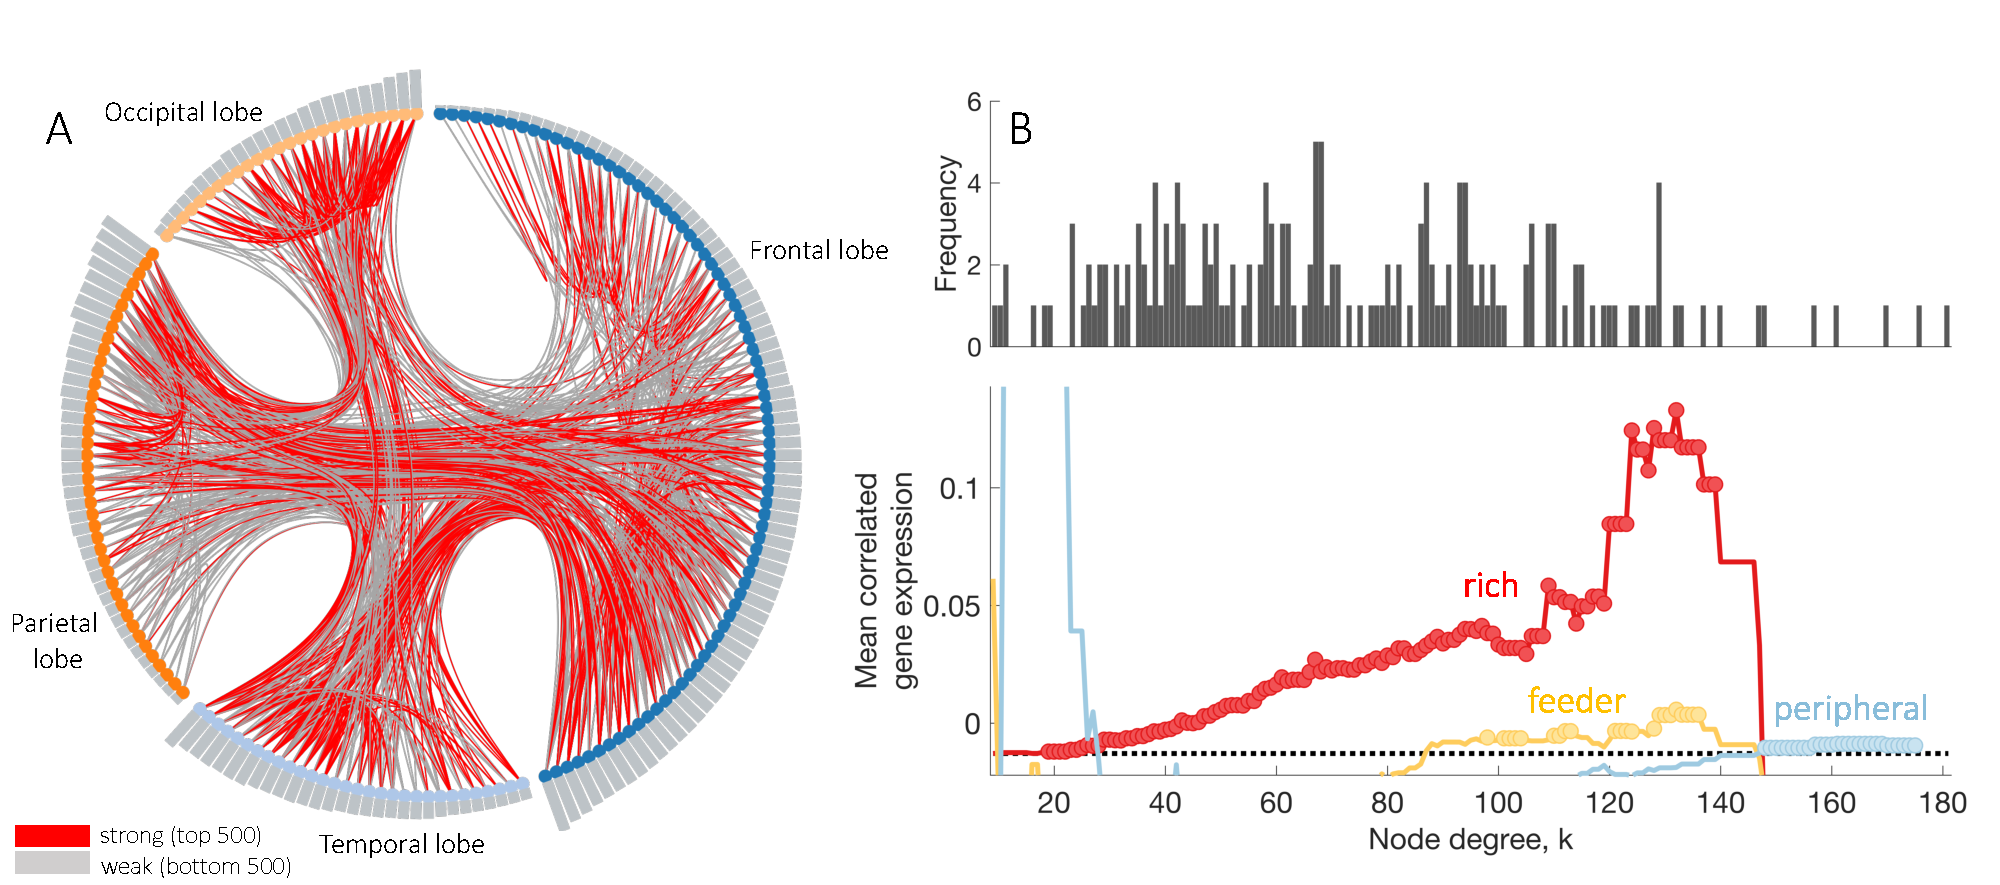
\includegraphics[width=1\textwidth]{Chapter5/Ch5Fig5.pdf}% This is a *.eps file
%https://immersive.erc.monash.edu/neuromarvl/?save=7ecb3a65-228e-4299-bcd4-2c65423741a8_130.194.90.94
\end{center}
\caption{\textbf{Rich links show distinct correlation patterns in relation to the genetic risk for disorders and genetic scores for IQ.}
Top: Degree distribution, \textit{k}, of the connectome. Bottom: Mean partial correlation (Spearman) coefficient between the connection weight and polygenic scores for schizophrenia (A), major depression (B), ADHD (C), ASD (D), bipolar disorder (E) and IQ (F) for each connection type as a function of \textit{k}. The mean partial correlation across all network links is shown as a dotted black line; Circles indicate a statistically significant decrease (A-E) and increase (F) in correlation coefficient in a given link type relative to the rest of the network (one-sided Welch's $t$-test, $p < 0.05$).}
\label{fig:Ch5Fig5}
\end{figure}

We also investigated the association between connectivity strength and polygenic scores for IQ expecting the opposite association, namely, that higher polygenic scores will be related to increased hub connectivity. First, we tested whether polygenic scores derived based on the latest publicly available GWAS for IQ \citep{Savage2018} were informative of the IQ scores in our sample. Indeed, the polygenic scores at $p_{T} = 0.05$ were able to explain $6.2\%$ variance in IQ measures in our sample ($p = 3.6 \times 10^{-7}$), comparable with previously found associations between PGS and phenotypic traits \citep{Euesden2015} suggesting a meaningful association with the phenotype. As shown in Figure \ref{fig:Ch5Fig5}F, the average correlation between the polygenic scores and connectivity strength was the highest for rich followed by feeder links while no increase was observed in peripheral connections. This relationship suggests a positive association between the genetic scores for IQ and connection strength between hubs. In other words, people with higher genetic scores for IQ, on average, have an increased connectivity strength for connections between hubs. Across the topological rich club regime ($k > 110$), the associations are stronger for rich compared to feeder links as well as for feeder compared to peripheral (Welch's $t$-test; all $p<0.01$).


Despite the association in all cases being relatively weak, the opposite relationships observed in the case of the polygenic scores for disorders and IQ imply a meaningful trend. Together, these results suggest that the effects of the structural DNA variation evaluated through the cumulative effect using polygenic scores converge on hubs and exemplify the same trend observed in the analysis of heritability.

\subsection{Transcriptional coupling}

Finally, we investigated the transcriptional properties of connectivity by evaluating the transcriptional coupling between brain regions, as quantified using CGE, across different link types. The analysis was focused to the left hemisphere due to the limited coverage of the AHBA (see section \nameref{secGeneExpression}). Figure \ref{fig:Ch5Fig6}A visualizes the anatomical distribution of connections between the region pairs with the strongest (highest positive CGE) and weakest (lowest absolute CGE) transcriptional coupling. The strongest transcriptional coupling is more likely to occur between higher degree nodes. To further investigate the patterns of transcriptional coupling between different link types, we plot the mean CGE for every link type as a function of degree threshold (Figure \ref{fig:Ch5Fig6}B). The plot reveals that CGE for rich links increases as a function of degree, with a sharp increase observed within the topological rich club regime. Feeder links showed only a very marginal increase at the highest degree thresholds, while peripheral links had the lowest CGE. These CGE findings thus mirror those obtained in the heritability and polygenic score analysis.

\begin{figure}[h!]
\begin{center}
\includegraphics[width=1\textwidth]{Chapter5/Ch5Fig6.pdf}% This is a *.eps file
%https://immersive.erc.monash.edu/neuromarvl/?save=7ecb3a65-228e-4299-bcd4-2c65423741a8_130.194.90.94
\end{center}
\caption{\textbf{Rich links show an increased correlated gene expression.}
(A) Connectogram showing the anatomical distribution of connections between the regions with the strongest (top 500 highest positive) and weakest (lowest absolute) transcriptional coupling. Connections (lines) between brain regions (circles) are coloured according to the correlated gene expression between the regions they connect. Brain regions are organised by the lobe (shown in node colour) and sorted by degree (shown in bars). 
(B) Top: The degree distribution of the left hemisphere group-level connectome. The degree for every region is based on the whole brain connectivity. Bottom: Mean CGE for `rich' (hub -- hub), `feeder' (hub -- non-hub), `peripheral' (non-hub -- non-hub) connections as a function of degree threshold, \textit{k} used to define hubs. The mean CGE across all network links shown as a dotted black line. Circles indicate a statistically significant increase in CGE in a given link type compared to the rest of the network (one-sided Welch's $t$-test, $p < 0.05$).}
\label{fig:Ch5Fig6}
\end{figure}

We next investigated whether any particular functional groups of genes are driving the transcriptional coupling between hubs. Each gene was assigned a score quantifying its contribution towards the increase in CGE in rich compared to peripheral links, as these two categories present the most topologically distinct connection types (see section \nameref{sec:CGE}). For this analysis edges within the topological rich club regime (degree $> 105$) were defined as rich and links between regions with degree $\leq105$ as peripheral. We performed a gene score resampling (GSR) analysis (see section \nameref{sec:enrichment}) to determine whether high-scoring genes were enriched in any gene ontology (GO) biological process categories. A total of 41 category showed a significant ($p<0.05$, FDR corrected) increase in the CGE for rich links. These categories included those related to cell metabolism including `ATP synthesis coupled electron transport', `oxidative phosphorylation', `cellular respiration' and `nucleotide phosphorylation', among others (see Figure \ref{fig:Ch5SFig14}). The involvement of metabolism-related genes in driving the increased CGE between hub regions is in line with their high energetic demands \citep{Bullmore2012,Collin2014,Liang2013a,Tomasi2013} and match previous analyses of CGE in mouse \citep{Fulcher2016}, and spatial gene-expression maps in human \citep{Vertes2016b}.

\section{Discussion}

Hubs are thought to represent costly but functionally valuable elements of brain networks \citep{VandenHeuvel2012} that demonstrate conserved organization across a range of species and scales \citep{Harriger2012,Towlson2013,VandenHeuvel2011,Zamora-Lopez2010}. Here we confirm that connections between hubs in the human brain are topologically central and costly, as previously demonstrated \citep{VandenHeuvel2012}, and show that hub connectivity is likely to be under tight genetic control. Specifically, we find that compared to the rest of the network, connections between hubs are more heritable; that hub regions display increased transcriptional coupling despite being separated by longer distances; that increased genetic risk for psychiatric disorders is associated with reduced hub connectivity; and higher genetic scores for IQ are related to increased connectivity strength between hubs. Together, these findings demonstrate a relationship between the large-scale brain connectivity and genetics, with the most pronounced effects on edges involving network hubs -- regions that are among the most costly and functionally valuable elements of the connectome.

Early genetic studies have successfully implemented heritability analyses to quantify genetic contributions towards a range of imaging derived phenotypes \citep{Colclough2017,Fornito2011,Peper2007,Roshchupkin2016,Shen2014,Sinclair2015,Sudre2017,Thompson2001}, demonstrating moderate to high degree of genetic influences. In line with the general principles of brain organisation suggesting a trade-off between minimising the wiring cost and maximising the communication efficiency, prior evidence of a strong genetic contribution towards regional cost-efficiency in functional networks \citep{Fornito2011} supports the hypothesis that brain networks have evolved to satisfy the competitive selection criteria of minimizing cost and promoting efficient, adaptive performance. Hub connectivity plays a central role in how nervous systems negotiate this trade-off \citep{VandenHeuvel2013b}  and, as our findings demonstrate, is under substantial genetic control. Indeed, the gradual increase in heritability for rich links followed by feeder connections across a range of degree thresholds indicates a graded nature of the effect such that the genetic control over brain connectivity is increasing with increasing topological connection centrality.

Having established that the contributions of additive genetic factors converge on connections between hubs we aimed to investigate how inter-individual differences in hub connectivity relate to the structural DNA variations between people. We evaluated the associations between polygenic scores for five major psychiatric disorders and structural connectivity and found that genetic susceptibility for illness is preferentially linked to reduced connection strength between hubs. Under the assumption that hubs form a putative backbone for brain communication \citep{Harriger2012,Towlson2013,VandenHeuvel2011,VandenHeuvel2013b}, decreased connectivity strength between them might indicate a reduced integrative capacity that is linked to the increased genetic predisposition to psychiatric disorders. Consistently negative associations across disorders were countered by the positive trend observed in relation to the polygenic scores for IQ indicating an increased connectivity strength between hubs in subjects with the higher genetic scores for IQ. Although the associations are moderate, consistent with the bulk of polygenic associations reported thus far \citep{Alloza2018,Dezhina2018,Liu2016a,Sadeh2018,Wang2017}, the opposite direction of the associations for disorders and IQ suggests that different genes exert opposing effects on hub connectivity, ultimately resulting in the expression of distinct behavioural phenotypes. Although, the utility of the polygenic scores in the field of imaging genetics has been questioned \citep{Reus2017}, a number of studies have identified associations between PGS and cortical gyrification \citep{Liu2016a}, functional connectivity \citep{Dezhina2018,Sadeh2018,Wang2017} and longitudinal changes in white matter properties \citep{Alloza2018}. More specifically, in line with the directionality of our results, genetic predisposition to major depression was found to be associated with decreased global white matter integrity \citep{Whalley2013} whereas higher genetic scores for IQ showed a positive association with global FA \citep{Jansen2018}. Our findings indicate that polygenic liability for psychiatric disorders, and genetic predisposition to adaptive traits such as IQ, is preferentially associated with functionally critical hub connectivity.

Next, we aimed to replicate the previous findings in mouse \citep{Fulcher2016} and \textit{C.elegans} \citep{Arnatkeviciute2018} demonstrating increased gene expression similarity between hubs. Investigating how gene expression patterns track macroscale brain network organisation in human became possible through the availability of the Allen Human Brain Atlas \citep{Hawrylycz2012}. In the past few years, a range of brain network properties in human have been related to gene expression \citep{Cioli2014b,Forest2017,Goel2014,Richiardi2015,Vertes2016b}. Replicating the previous findings in mouse \citep{Fulcher2016} and \textit{C.elegans} \citep{Arnatkeviciute2018}, consistently increasing CGE between hubs suggests some intrinsic genetic similarity between those regions despite their disparate anatomical locations. Moreover, the involvement of metabolism-related genes in driving this transcriptional coupling mirrors the findings in both mouse \citep{Fulcher2016} and human \citep{Vertes2016b} indicating a conserved transcriptional signature supporting high energetic requirements of hub areas \citep{Liang2013a,Tomasi2013} that transcends different species. This result is consistent with evidence that hubs are metabolically expensive \citep{Vaishnavi2010,Varkuti2011}. Indeed, the high metabolic demands of hub regions may increase their sensitivity to metabolic distress, making these areas vulnerable to the effects of injury or disease \citep{Crossley2014,Fornito2015}. It is possible that CGE of metabolic genes may be related to similarities in the microcircuitry of hub regions, given that the AHBA data are derived from bulk tissue samples and do not distinguish expression patterns of different cell types. Single-cell sequencing \citep{Lein2017} would shed some light on this possibility.

Providing such unprecedented opportunities for new research, the usage of publicly available databases such as AHBA pose several challenges as integrating gene expression measures derived from an atlas together with imaging data requires substantial consideration \citep{Arnatkeviciute2019,Fornito2019}. One of the most critical aspects in investigating the transcriptional correlates of a spatially varying brain imaging phenotype such as connectivity, are the spatial properties of gene expression. Spatial autocorrelations of gene expression have been observed across multiple species \citep{Arnatkeviciute2018,Burt2018,Fornito2019,Fulcher2016} with regions in close proximity exhibiting more similar gene expression. Whereas spatial autocorrelation of gene expression is an interesting question in itself, most studies relating gene expression to the imaging derived phenotypes aim to evaluate the relationships beyond simple spatial patterns. This can be achieved by statistically controlling for these relationships \citep{Fakhry2015a,Fulcher2016} or by evaluating the statistical significance of the result based on the spatially constrained null models \citep{Burt2018,Romero-Garcia2018,Whitaker2016a,Vasa2018,Vertes2016b}. Here we account for the spatial relationship by approximating it with an exponential trend and analysing the spatially corrected CGE as the residuals from a bulk spatial trend estimated as an exponential fitted to all pairs of brain regions. Therefore, the observed transcriptional similarity between hub regions does not result from the general spatial trends in gene expression and thus provides additional information regarding their functional role.

\section{Conclusions}
In this work we combined three different approaches spanning several levels of genetic inference to systematically evaluate genetic contributions to brain connectivity. We demonstrate that functionally important connections between topologically central network hubs are under stronger genetic control compared to more topologically peripheral links. At the level of structural DNA variation, we show that polygenic liability for psychiatric disorders is preferentially associated with decreased connectivity strength between hubs whereas higher polygenic scores for IQ are indicative of increased hub connectivity. Linking gene function and brain-wide connectivity we show that hub regions display a tightly coupled gene expression. This transcriptional coupling is driven by metabolism-related genes. Together, our findings demonstrate a direct link between molecular function and the large-scale organisation of the human connectome.
